\section{Settings}\label{sprint3:settings}

Since the requirements has not changed at all since last sprint, the ones regarding settings remain the same.
During this sprint the following requirements were handled; \ref{sprint2_database_req}, \ref{sprint2:req:calibrate}, \ref{sprint2:req:picto_gauge}, and \ref{sprint2:req:speed} (see \cref{sprint3:requirement_table}).

The settings activity still handles the same three things as previously; speed of the car, garage colors, and calibration of the microphone.
The method for changing the speed and garage colors was changed during this sprint.
Calibration of the microphone was not changed, as no proper solution was found this sprint.
A screenshot of the settings activity can be seen in \cref{sprint3:settings:screenshot}.

\begin{figure}
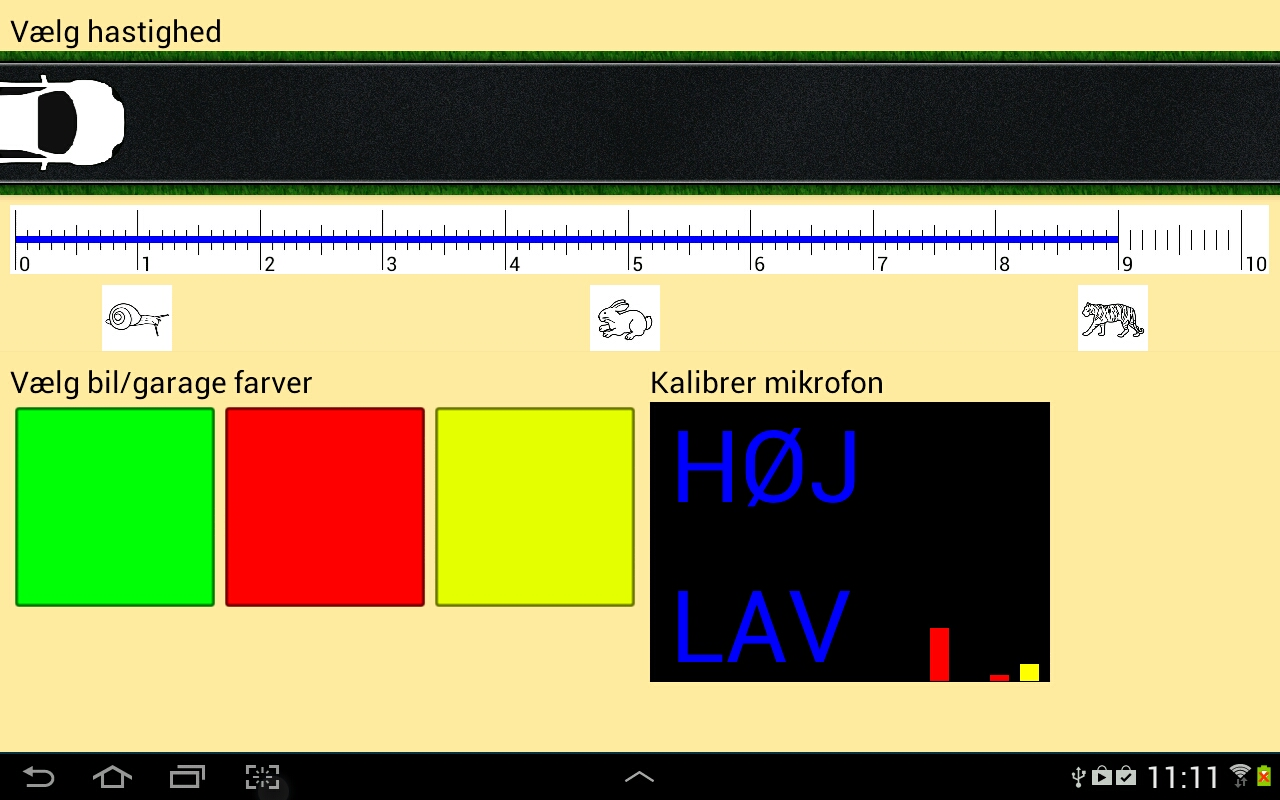
\includegraphics[width=\textwidth]{sprint3/settings_screenshot}
\caption{Screenshot of the Settings activity}
\label{sprint3:settings:screenshot}
\end{figure}

\paragraph{Altering of Speed} was changed according to requirements \ref{sprint2:req:picto_gauge} and \ref{sprint2:req:speed}.
The speed is set by either pressing the gauge, changing the position of the gauge-bar, which indicates the currently set speed.
Alternatively the pictograms (currently three; snail, rabbit, and tiger) can be pressed, moving the gauge-bar and setting the speed appropriately.

\paragraph{Choosing garage colors} is now depicted as a colored box, where the box's color is corresponding to the selected garage color.
A color can then be changed by pressing one of these boxes and choosing a new one from a color-picker (see \cref{sprint3:gui}).